\subsubsection{Increased instrument-shaft resistance}
\label{sec:shaft_resistance_results}

\paragraph{Parameter distributions and associations}
Figure~\ref{fig:dof2-box} compares selected current-residual and video
parameters across command amplitudes. The M1 absolute current-residual peak
separated the recorded groups at each amplitude, whereas M2 phase mean
and second-harmonic amplitude depended strongly on command amplitude.
The pooled Pearson matrix in Figure~\ref{fig:dof2-corr} describes
associations between extracted parameters. These associations may reflect
both class differences and amplitude effects; within-class and
amplitude-specific matrices are provided in Appendix~\ref{app:dof2}.

\begin{figure*}[t]
\centering
\includegraphics[width=0.8\textwidth]{Figures/01_parameter_boxplots.pdf}
\caption{Selected DOF2 residual parameters by command amplitude.
Each point is the mean of three per-cycle parameter values from one
command condition. Colours identify healthy and degraded observations;
markers distinguish runs. Boxes show the median and interquartile range.
Whiskers extend to the most extreme observations within 1.5 interquartile
ranges. All observations are shown. Blocks from one run are not independent
experiments.}
\label{fig:dof2-box}
\end{figure*}

\begin{figure*}[t]
\centering
\includegraphics[width=0.75\textwidth]{Figures/02_parameter_correlations.pdf}
\caption{Pearson correlations between selected three-cycle parameters,
pooled over classes and amplitudes. These are correlations between
parameters across observations, rather than between waveforms within a
cycle. Class and amplitude effects may contribute to the correlations.}
\label{fig:dof2-corr}
\end{figure*}

\paragraph{Cross-validation and observation length}
Table~\ref{tab:dof2-overall} reports complete-run cross-validation for
single-cycle observations and three-cycle feature means.
One cycle contains both positive and negative commanded bending and
returns to its starting phase. Each parameter is first calculated from
all valid samples in that cycle. For three-cycle observations, the three
parameter vectors from consecutive cycles of the same waveform,
frequency and amplitude are averaged. Waveforms are not averaged before
parameter extraction, and different amplitudes are not averaged together.

Each run contains 18 command conditions and three cycles per condition.
The four runs therefore provide 216 single-cycle observations
(108 per class), or 72 three-cycle observations (36 per class).
In each validation fold, one complete run is withheld and the other three
runs are used for standardisation and LDA fitting.
The pooled model uses conditions at all three amplitudes, frequencies and
both waveforms together. The standard decision boundary is $d=0$.

\begin{table}[t]
\centering
\caption{Pooled shaft LDA cross-validation for one-cycle and three-cycle observations, with 108 and 36 observations per class, respectively. Each complete run is held out once. Green highlights the selected M1 absolute-peak model. Counts are repeated observations from two runs per class.}
\label{tab:dof2-overall}
\scriptsize
\setlength{\tabcolsep}{2.5pt}
\resizebox{\columnwidth}{!}{%
\begin{tabular}{>{\raggedright\arraybackslash}p{2.6cm} cccc !{\color{black!25}\vrule width 0.4pt} cccc}
\toprule
 & \multicolumn{4}{c}{\textbf{1 cycle}} & \multicolumn{4}{c}{\textbf{3 cycles}} \\
\cmidrule(lr){2-5} \cmidrule(lr){6-9}
\textbf{Parameters} & TP & FP & TN & FN & TP & FP & TN & FN \\
\midrule
M1 absolute peak & \gbcorrect{108} & \gbcorrect{0} & \gbcorrect{108} & \gbcorrect{0} & \gbcorrect{36} & \gbcorrect{0} & \gbcorrect{36} & \gbcorrect{0} \\
M1 RMS & 108 & 0 & 108 & 0 & 36 & 0 & 36 & 0 \\
M2 phase mean & 82 & 0 & 108 & 26 & 27 & 0 & 36 & 9 \\
M2 second harmonic & 81 & 0 & 108 & 27 & 28 & 0 & 36 & 8 \\
M2 RC & 54 & 3 & 105 & 54 & 18 & 1 & 35 & 18 \\
Absolute gain diff. & 76 & 8 & 100 & 32 & 24 & 2 & 34 & 12 \\
Positive/negative gains & 106 & 19 & 89 & 2 & 36 & 6 & 30 & 0 \\
Centred video MAE & 86 & 15 & 93 & 22 & 28 & 5 & 31 & 8 \\
M1 peak + gain diff. & 108 & 0 & 108 & 0 & 36 & 0 & 36 & 0 \\
M2 mean + gain diff. & 74 & 4 & 104 & 34 & 25 & 1 & 35 & 11 \\
M2 harmonic + gain diff. & 81 & 2 & 106 & 27 & 26 & 0 & 36 & 10 \\
M2 harmonic + video MAE & 69 & 8 & 100 & 39 & 23 & 3 & 33 & 13 \\
\bottomrule
\end{tabular}%
}
\end{table}


M1 absolute peak and M1 RMS correctly classified all held-out
observations at both observation lengths. For the three-cycle models,
M2 phase mean detected 27/36 degraded observations and M2 second harmonic
28/36, without false alarms. M2 RC detected 18/36, with one false alarm.
For the three-cycle M1-peak-only classifier, the four fold-specific thresholds ranged
from 67.28 to 68.80~mA of current residual.

Video-only performance depended on the selected representation.
Absolute gain difference detected 24/36 degraded observations with
2/36 false alarms. Using positive and negative gain together detected
36/36 with 6/36 false alarms. Centred video-residual MAE detected 28/36
with 5/36 false alarms. Adding a video parameter did not consistently
improve the pooled M2 models.

\paragraph{Pooled current-only LDA}
Figure~\ref{fig:dof2-lda} shows one current-only LDA model using
M1 absolute current-residual peak and M2 current-residual RMS.
All amplitudes are included in the same fit. The 72 points remain
separate three-cycle observations; no additional averaging is performed
across amplitudes, frequencies or runs. The model directly uses the two
standardised parameters without PCA.
This fit illustrates the feature geometry; the held-out results in
Table~\ref{tab:dof2-overall} come from separate validation-fold models.
The two-parameter boundary in this figure is distinct from the scalar
M1-peak-only thresholds reported above.

\begin{figure}[t]
\centering
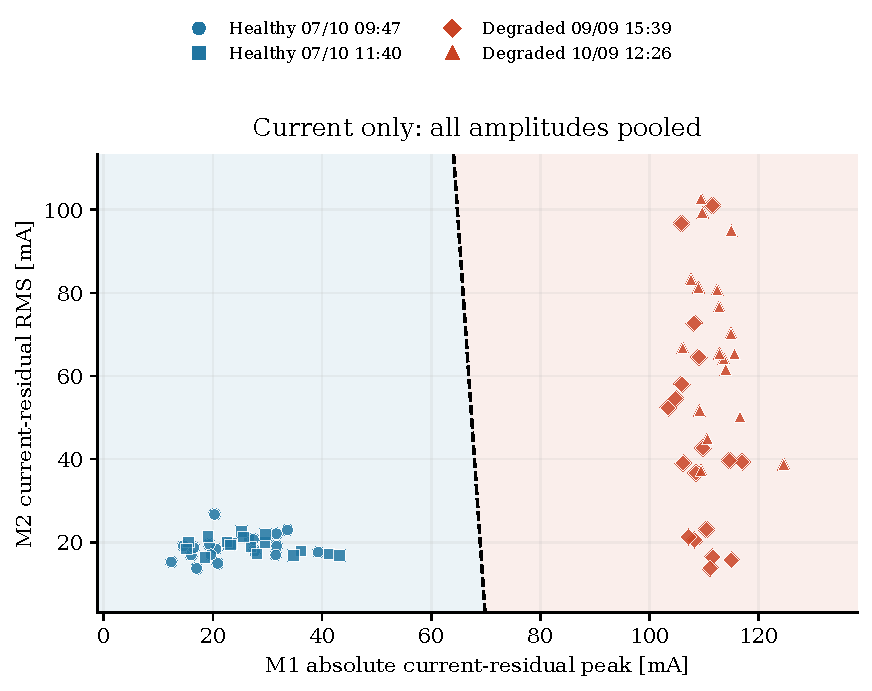
\includegraphics[width=0.98\columnwidth]{Figures/03_pooled_current_lda.pdf}
\caption{Descriptive current-only LDA using M1 absolute current-residual
peak and M2 current-residual RMS. Small, medium and full amplitudes are
pooled in one model. Each point is a separate three-cycle feature mean;
colours distinguish classes and markers distinguish runs.
The dashed line is the boundary of the model fitted to all 72 displayed
observations. This is a descriptive fit, not a cross-validation boundary.}
\label{fig:dof2-lda}
\end{figure}

\paragraph{Amplitude dependence and whole-run decisions}
Separate amplitude-specific models are reported in
Table~\ref{tab:dof2-amplitude}. At small amplitude, combining M2 second
harmonic with gain difference increased detection from 6/12 to 9/12,
while adding one false alarm. At medium and full amplitude, this pair
detected 12/12 with no false alarms. M1 absolute peak already detected
12/12 without false alarms at every amplitude. The added value of video
was therefore conditional on the current parameter and amplitude.

The fixed sensitivity-oriented threshold comparison is provided in
Table~\ref{tab:dof2-alarm}. It uses the same held-out scores and changes
only the decision threshold. Whole-run decisions average the 18 held-out
condition scores before applying the threshold; these are four run-level
decisions, distinct from the 72 condition-level decisions above.

These findings describe two healthy and two degraded runs.
Recording date and potentially shaft orientation or mounting are
confounded with class. The results demonstrate separation of the available
recordings and do not establish a friction-specific or guaranteed future
detection rate.
